\documentclass[preprint,11pt]{elsarticle}
\usepackage{amsmath,amssymb,amsthm}
\usepackage{chngcntr}
\usepackage{booktabs,array}
\usepackage{graphicx}
\usepackage{float}
\usepackage{xcolor}
\usepackage{tikz}
\usetikzlibrary{arrows.meta,positioning,shapes.geometric,calc}
\usepackage{pgfplots}
\pgfplotsset{compat=1.18}
\usepackage[hidelinks]{hyperref}
\usepackage{xurl}
\usepackage{fontspec}
\setlength{\emergencystretch}{3em}
\biboptions{numbers,sort&compress}
\newtheorem{theorem}{Theorem}
\newtheorem{definition}{Definition}
\journal{Knowledge-Based Systems}

\begin{document}
\begin{frontmatter}
\title{A Decision-Diagnostic Framework for Incomplete Machine Learning Leaderboards: Evidence Ambiguity versus Certificate Failure under Task Reweighting}

\author[hct]{Ghassan Malkawi\corref{cor1}}
\ead{gmalkawi@hct.ac.ae}
\author[cud]{Ahmed Elsayed}
\ead{ahmed.elsayed@cud.ac.ae}
\author[uaeu]{Mohammed Alhagyan}
\ead{m.alhagyan@uaeu.ac.ae}
\author[scc]{Bakeel Hussein}
\ead{bakeel.almaher@scc.edu.ye}

\cortext[cor1]{Corresponding author.}
\affiliation[hct]{organization={Faculty of Computer Information Science, Higher Colleges of Technology}, addressline={Al Ain Campus, P.O. Box 17155}, city={Al Ain}, country={United Arab Emirates}}
\affiliation[cud]{organization={Department of Computer Engineering and Computational Sciences, Canadian University Dubai}, addressline={P.O. Box 117781}, city={Dubai}, country={United Arab Emirates}}
\affiliation[uaeu]{organization={Department of Mathematical Sciences, College of Science, United Arab Emirates University}, addressline={P.O. Box 15551}, city={Al Ain}, country={United Arab Emirates}}
\affiliation[scc]{organization={Department of Applied Engineering, Sana'a Community College}, city={Sana'a}, postcode={5695}, country={Yemen}}

\begin{abstract}
Incomplete multi-task machine-learning leaderboards can remain unresolved for different logical reasons, so a decision-support process should diagnose the source of non-resolution before requesting more evaluation. We study normalized-rank leaderboards whose task weights vary within a total-variation neighborhood and distinguish information-limited, certificate-limited, certified/resolved, and inconclusive states. Exact constructions establish certificate-limited states, including a 68-task uniform-center construction with independently admissible unknown folds, 65,780 canonical states, and 789,360 exact ordered support comparisons. In a TabArena study with 51 tasks, 14 methods, and 816 paired fold vectors, opposite-answer completions prove information limitation at 47 of 80 immediate pre-stopping prefixes. For all 47 witnessed traces, ambiguity immediately before the recorded stopping prefix together with a verified stopping-prefix certificate identifies that prefix as the first semantically resolvable point along the recorded disclosure order; the remaining 33 traces are inconclusive. A tested certificate strengthening yields no earlier stopping across 480 prespecified checkpoints. The framework therefore distinguishes when additional benchmark evidence is logically necessary from when the reasoning mechanism, rather than the evidence, is the limiting component.
\end{abstract}

\begin{keyword}
machine-learning evaluation \sep decision diagnosis \sep incomplete benchmarks \sep robust model selection \sep task reweighting \sep information sufficiency
\end{keyword}
\end{frontmatter}

\section{Introduction}

Multi-task machine-learning benchmarks increasingly guide model selection, deployment shortlists, and claims of state-of-the-art performance. Yet a leaderboard may have to support a decision while fold evaluations are still undisclosed, some evaluations are unavailable, or task priorities remain contestable. An unresolved leaderboard therefore poses a decision-support question before it poses a data-collection question: what, exactly, prevents the available evidence from supporting a defensible decision?

Two distinct barriers are possible. In an information-limited state, two completions consistent with every disclosed evaluation yield opposite decisions; no sound analysis can choose between them without additional evidence or stronger assumptions. In a certificate-limited state, every compatible completion yields the same decision, but the chosen proof device cannot certify it; collecting more evaluations may then be unnecessary. A third outcome must also be preserved: when neither an opposite-answer pair nor semantic determination has been established, the correct label is inconclusive rather than implicitly resolved.

This paper develops a sound decision-diagnostic framework for these states in rank-based multi-task leaderboards with fold-level observations and task weights that may vary within a total-variation (TV) neighborhood. A diagnostic label is assigned only when the corresponding witness or proof is available; otherwise the state remains explicitly inconclusive. Figure~\ref{fig:diagnostic_logic} summarizes this logic.

\begin{figure}[t]
\centering
\resizebox{0.98\linewidth}{!}{%
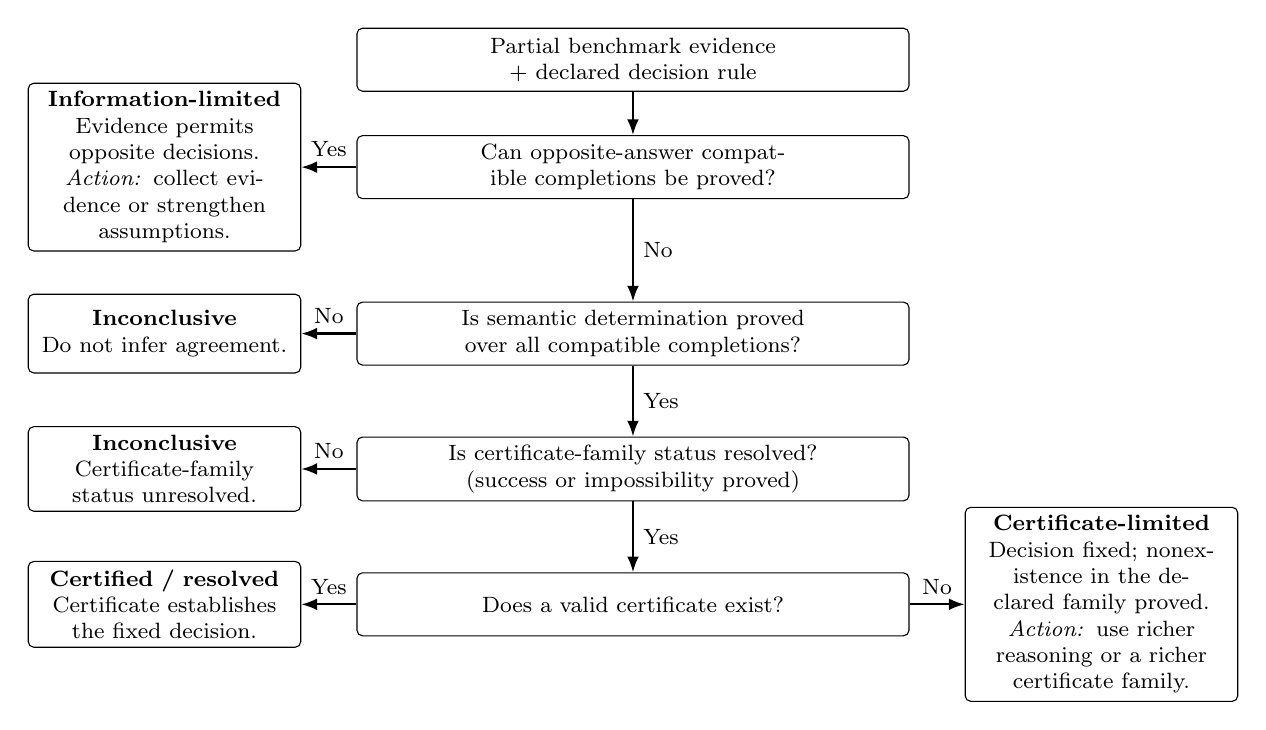
\begin{tikzpicture}[
  node distance=5.5mm and 9mm,
  every node/.style={font=\footnotesize,align=center},
  q/.style={draw,rounded corners=2pt,text width=6.8cm,minimum height=8mm,inner sep=3pt},
  outcome/.style={draw,rounded corners=2pt,text width=3.25cm,minimum height=10mm,inner sep=3pt},
    arr/.style={-{Latex[length=2mm]},thick}
]
\node[q] (start) {Partial benchmark evidence + declared decision rule};
\node[q,below=of start] (q1) {Can opposite-answer compatible completions be proved?};
\node[q,below=13mm of q1] (q2) {Is semantic determination proved over all compatible completions?};
\node[q,below=9mm of q2] (q3) {Is certificate-family status resolved?\\(success or impossibility proved)};
\node[q,below=9mm of q3] (q4) {Does a valid certificate exist?};

\node[outcome,left=7mm of q1] (info) {\textbf{Information-limited}\\Evidence permits opposite decisions.\\\emph{Action:} collect evidence or strengthen assumptions.};
\node[outcome,left=7mm of q2] (inc1) {\textbf{Inconclusive}\\Do not infer agreement.};
\node[outcome,left=7mm of q3] (inc2) {\textbf{Inconclusive}\\Certificate-family status unresolved.};
\node[outcome,left=7mm of q4] (cert) {\textbf{Certified / resolved}\\Certificate establishes the fixed decision.};
\node[outcome,right=7mm of q4] (clim) {\textbf{Certificate-limited}\\Decision fixed; nonexistence in the declared family proved.\\\emph{Action:} use richer reasoning or a richer certificate family.};

\draw[arr] (start)--(q1);
\draw[arr] (q1)--node[above]{Yes}(info);
\draw[arr] (q1)--node[right]{No}(q2);
\draw[arr] (q2)--node[above]{No}(inc1);
\draw[arr] (q2)--node[right]{Yes}(q3);
\draw[arr] (q3)--node[above]{No}(inc2);
\draw[arr] (q3)--node[right]{Yes}(q4);
\draw[arr] (q4)--node[above]{Yes}(cert);
\draw[arr] (q4)--node[above]{No}(clim);
\end{tikzpicture}%
}
\caption{Sound decision-diagnostic logic for partial benchmark evidence. An explicit pair of compatible completions with opposite decisions proves information limitation. Certificate limitation requires both semantic determination and a proof that no valid certificate exists in the declared family. Failure of an incomplete witness or certificate search remains inconclusive.}
\label{fig:diagnostic_logic}
\end{figure}

The theoretical and empirical components answer complementary parts of this diagnostic problem. Exact constructions test certificate expressiveness over all compatible completions. The real TabArena study tests information sufficiency along fixed disclosure traces using only disclosed fold vectors and declared completion domains. The same decision predicate and task-weight neighborhood connect both components.

The contribution couples three ingredients: missing observations at the fold level, uncertainty in task importance represented by a TV neighborhood, and the robust common-weak-winner decision over all admissible task weights. Within that setting, we prove that semantic determination need not be representable by the completion-independent joint-mixture certificate family studied here, and we separately show on real benchmark transcripts when the disclosed evidence itself admits opposite decisions. The resulting contribution is diagnostic: it separates limits of the available evidence from limits of the declared certificate family.

The main findings are fourfold. First, the diagnostic framework separates evidence ambiguity, certificate failure, certified resolution, and inconclusive states without treating failed searches as evidence of agreement. Second, a completion-independent fixed joint-mixture certificate is not complete for the studied leaderboard decision: every compatible completion can agree while the certificate still fails. This obstruction persists in a 68-task construction with uniform nominal weights and independently admissible unknown folds; exhaustive symmetry reduction checks 65,780 canonical states and 789,360 ordered support comparisons. Third, the real-data study proves information limitation at 47 of 80 immediate pre-stopping prefixes. For each of those 47 traces, the ambiguity witness at $Q-1$ and the verified certificate at $Q$ form a fixed-trace lower/upper match, identifying $Q$ as the first semantically resolvable disclosure count along that recorded order within the stated numerical scope. The other 33 traces remain inconclusive. Fourth, the tested certificate strengthening yields no earlier stopping at any of 480 sampled checkpoints.

\section{Related work and positioning}

Incomplete benchmark evaluation is already an established research problem. Himmi et al. \cite{r1} study missing system scores in natural language processing benchmarks by mapping observed scores to compatible partial rankings and aggregating completed rankings with Borda-style procedures. Their objective is to obtain robust aggregate rankings when evaluations are absent. Our objective is different: we do not impute one ranking and then aggregate it. We ask what decision statements are logically supported by all benchmark completions that remain compatible with the disclosed fold-level evidence.

Possible and necessary winners under partial preference information are classical problems in computational social choice. Xia and Conitzer \cite{r2} characterize when a candidate can or must win across completions of partial orders. Lu and Boutilier \cite{r3} develop robust winner determination and preference-elicitation procedures under partial rankings using minimax regret. These works establish the general semantics of reasoning over incomplete preference information.

Uncertainty over weights is also established. Baumeister et al. \cite{r4} study possible winners when voter weights are uncertain, including rational and integer weights and variants with ranges and total-weight bounds. Viappiani \cite{r5} studies robust winner determination for positional scoring rules when scoring-rule weights are uncertain, using minimax regret. O'Shea et al. \cite{r6} derive precise weight-stability intervals for the weighted-sum model.

The general concept of information certificates is likewise established. Parkes \cite{r7} formalizes minimal information certificates in combinatorial auctions. Corrente, Greco, and S\l{}owi\'nski \cite{r8} show how robust ordinal regression can incorporate imprecise evaluations, while decision-dependent information discovery studies optimization in which information becomes available only after a deliberate action \cite{r9}.

Recent machine-learning work makes the benchmark-specific connection especially important. Mishra and Arunkumar \cite{r10} show that model rankings can change under alternative weighting and customization schemes. Gordienko et al. \cite{r11} formulate multi-task benchmarking as a social-choice problem and define an instance-level robustness quantity based on the number of benchmark tasks that must be manipulated to promote a target model. TabArena \cite{r12} provides the real benchmark setting used in our study. Our object differs from these studies in combining fold-level partial evidence, a total-variation neighborhood of task importance, and a completion-independent certificate for a common-weak-winner decision.

A broader machine-learning benchmarking literature shows that conclusions depend on task selection, repetitions, uncertainty, and reporting. Multi-dataset comparison protocols \cite{r13,r14} and benchmark-variance analyses \cite{r15} motivate caution when interpreting aggregate rankings. OpenML and its benchmarking suites \cite{r16,r17}, together with AMLB, an automated machine-learning benchmark \cite{r18}, emphasize standardized tasks, reproducible splits, explicit failures, and reusable benchmark evidence. These works motivate our fixed disclosure units and provenance, but they do not address the certificate-versus-information distinction studied here.

Weight-space uncertainty and necessary/possible conclusions also have a long multiple-criteria decision analysis (MCDA) history. Stochastic multicriteria acceptability analysis (SMAA) and SMAA-2 explore which weight vectors support alternatives or ranks under uncertain preference information \cite{r19,r20}, with later work addressing computational implementation \cite{r21}. Robust ordinal regression constructs necessary and possible relations over all compatible preference models \cite{r22,r23,r24}. These are close conceptual precedents; our theorem concerns a different object---a restricted completion-independent certificate over partially observed machine-learning rank tables under a TV-bounded task-weight neighborhood.

These literatures establish the broader foundations. Our contribution is a decision-diagnostic framework for partially observed machine-learning leaderboards, a certificate obstruction under TV-bounded task weights, and real-benchmark transcripts with verified opposite-answer completions.

\section{Observation model and robust leaderboard decision}

Let $D$ be the number of benchmark tasks and $M$ the number of compared methods. For task $d\in\{1,\ldots,D\}$, method $m\in\{1,\ldots,M\}$, and fold $k\in\{1,\ldots,N_d\}$, let $x_{dkm}$ denote the lower-is-better loss of method $m$ on fold $k$ of task $d$. A complete benchmark is $X=(x_{dkm})$. A disclosure transcript $h$ records the fold vectors observed so far, and the completion set $\mathcal X(h)$ contains every complete loss array that agrees with $h$ and with the declared score domains. This set is the evidence model over which all subsequent decision statements are evaluated.

For task $d$ and method $m$, let $a_{dm}(X)$ denote the declared aggregate of its fold losses. In the exact constructions, $a_{dm}$ is the arithmetic mean over real-valued folds. In the real-data study, aggregation follows the fixed source-order numerical reduction used in the real-data analysis. Keeping these targets separate prevents floating-point implementation details from being mistaken for the exact-real theorem.

To compare methods across tasks with different loss scales, rank the $M$ aggregate values $a_{d1}(X),\ldots,a_{dM}(X)$ within each task $d$; ties receive their usual average rank. Let $\operatorname{midrank}_d(a_{dm}(X))$ denote that within-task midrank and define
\begin{equation}\label{eq:rank}
R_{dm}(X)=\frac{\operatorname{midrank}_d(a_{dm}(X))-1}{M-1}.
\end{equation}
Thus $R_{dm}=0$ denotes the best rank and $R_{dm}=1$ the worst; exact ties receive the same intermediate value. Equation~\eqref{eq:rank} removes score scale but preserves only within-task ordering, so it does not measure the magnitude of performance differences.

For candidate and rival indices $i,j\in\{1,\ldots,M\}$ with $j\ne i$, define the weighted rank gap under task weights $w$ by
\begin{equation}\label{eq:gap}
G_{ij}(X,w)=\sum_{d=1}^{D} w_d\bigl(R_{di}(X)-R_{dj}(X)\bigr).
\end{equation}
Because lower rank is better, $G_{ij}>0$ means that $j$ has the better weighted rank, $G_{ij}=0$ is a tie, and $G_{ij}<0$ favors $i$. This sign convention is used throughout the theorem statements and the real-data witness checks.

Task importance is allowed to vary around a nominal weight vector $p$ in the probability simplex. For a total-variation (TV) radius $\varepsilon\ge0$, the admissible neighborhood is
\begin{equation}\label{eq:tv}
\mathcal W(p,\varepsilon)=\left\{w\in\mathbb R_+^D:\sum_{d=1}^{D}w_d=1,\;\frac12\lVert w-p\rVert_1\le\varepsilon\right\}.
\end{equation}
Here $\mathbb R_+^D$ denotes the nonnegative orthant and $\lVert\cdot\rVert_1$ is the $\ell_1$ norm. The quantity $\varepsilon$ is the amount of task-weight mass that may be redistributed, not a confidence level. When $\varepsilon=0$, $\mathcal W(p,\varepsilon)$ contains only $p$; increasing $\varepsilon$ permits larger changes in task priorities while preserving nonnegative weights that sum to one. For a fixed completion $X$ and ordered pair $(i,j)$, we call $\max_{w\in\mathcal W(p,\varepsilon)}G_{ij}(X,w)$ the \emph{support value}.

For a complete benchmark $X$, method $i$ is a common weak winner if it is never strictly worse than any rival anywhere in the declared weight neighborhood:
\begin{equation}\label{eq:cww}
G_{ij}(X,w)\le 0\qquad \forall w\in\mathcal W(p,\varepsilon),\;\forall j\ne i.
\end{equation}
Under partial evidence $h$, the negative decision ``no common weak winner'' is semantically determined when
\begin{equation}\label{eq:semantic}
\forall X\in\mathcal X(h),\;\forall i,\;\exists w\in\mathcal W(p,\varepsilon),\;\exists j\ne i:\;G_{ij}(X,w)>0.
\end{equation}
The witnesses $w$ and $j$ in Equation~\eqref{eq:semantic} may depend on both the candidate and the completion. This dependence is precisely what the restricted certificate studied in Section~5 removes.

\section{Decision-diagnostic framework}

To make the evidence-versus-certificate distinction operational, define the binary decision predicate
\begin{equation}\label{eq:decision_predicate}
\mathcal D(X)=
\begin{cases}
1, & \text{if }X\text{ has no common weak winner over }\mathcal W(p,\varepsilon),\\
0, & \text{otherwise.}
\end{cases}
\end{equation}
Equation~\eqref{eq:decision_predicate} turns each compatible completion into the decision label of interest. The diagnostic labels concern how this label behaves over the completion set $\mathcal X(h)$, not how likely any completion is.

\begin{definition}[Information-limited state]
A partial state $h$ is information-limited when there exist $X^{(a)},X^{(b)}\in\mathcal X(h)$ such that $\mathcal D(X^{(a)})\ne\mathcal D(X^{(b)})$. An explicit opposite-answer pair is therefore a sound certificate that the disclosed evidence does not determine a unique decision.
\end{definition}

\begin{definition}[Certificate-limited state]
For a specified sound certificate family $\mathcal C$, a partial state $h$ is certificate-limited when $\mathcal D(X)$ is constant over all $X\in\mathcal X(h)$, and nonexistence of a valid certificate in $\mathcal C$ for that fixed decision is established. An unsuccessful or incomplete certificate search is not sufficient for this label.
\end{definition}

The distinction is intentionally asymmetric. A single opposite-answer pair proves information limitation, whereas failure to find such a pair does not prove semantic determination. We therefore retain a third label, \emph{inconclusive}, whenever neither information limitation nor semantic determination has been established. A fourth outcome, \emph{certified/resolved}, occurs when the declared certificate establishes the fixed decision.

\paragraph{Sound diagnostic procedure.}
Given $h$, $p$, $\varepsilon$, and a declared certificate family, the decision-support logic is:
\begin{enumerate}
\item Search for two compatible completions with opposite values of $\mathcal D$. If one pair is verified, return \emph{information-limited}.
\item Otherwise, attempt to establish that $\mathcal D(X)$ is constant for all $X\in\mathcal X(h)$. If this is not established, return \emph{inconclusive}.
\item If semantic determination is established, evaluate the declared certificate family. If a valid certificate is found, return \emph{certified/resolved}. If nonexistence of such a certificate in the declared family is proved, return \emph{certificate-limited}. If neither success nor impossibility is established, return \emph{inconclusive}.
\end{enumerate}
The procedure is sound but may be incomplete when any search or determination step is incomplete. The joint-mixture certificate studied in Section~5 is one-sided and certifies only the $\mathcal D(X)=1$ outcome. Accordingly, the 33 unresolved real-data traces remain inconclusive, whereas the exact constructions establish certificate-limited states analytically.

\paragraph{Illustrative reading of the diagnostic.}
Suppose a partial transcript admits two legal completions that agree on every disclosed fold vector but satisfy $\mathcal D(X^{(a)})=0$ and $\mathcal D(X^{(b)})=1$. The missing information is then decision-relevant, so a sound workflow must request additional evidence or stronger assumptions rather than a more elaborate proof device. By contrast, Theorem~\ref{thm:uniform} provides a documented certificate-limited case: every legal completion has $\mathcal D=1$, yet the specified completion-independent joint-mixture family cannot certify that fact. There the evidence is already semantically sufficient for the decision, and the appropriate target is the reasoning object rather than additional benchmark disclosure. The example is diagnostic rather than an evaluation-cost optimization result.

\section{A restricted certificate and exact obstructions}

Semantic determination in Equation~\eqref{eq:semantic} allows a different defeating weight and rival for each compatible completion. We now test whether a simpler completion-independent proof object is always sufficient. For each candidate $i$, let $\mu_i$ be a probability distribution over joint actions $(w,j)$, where $w\in\mathcal W(p,\varepsilon)$ and $j\ne i$. The distribution is selected once and cannot depend on the unknown completion.

The restricted certificate excludes candidate $i$ if
\begin{equation}\label{eq:certificate}
\mathbb E_{(w,j)\sim\mu_i}\!\left[G_{ij}(X,w)\right]>0\qquad \forall X\in\mathcal X(h).
\end{equation}
If such a $\mu_i$ exists for every candidate, then every compatible completion has no common weak winner, so the certificate is sound. The converse is the substantive question: does semantic determination in Equation~\eqref{eq:semantic} always imply the existence of these completion-independent mixtures? Theorems~\ref{thm:nonuniform} and~\ref{thm:uniform} show that it does not.

\begin{theorem}[Nonuniform fixed-mixture obstruction]\label{thm:nonuniform}
There exists a bounded whole-fold disclosure state with four methods labeled A--D and four tasks, exact arithmetic means, exact normalized midranks, nominal weights $p=(21,21,21,5)/68$, and $\varepsilon=13/400$ such that every compatible completion has no common weak winner, yet no completion-independent joint mixture satisfies the certificate for candidate A.
\end{theorem}

The construction uses one partially observed task and three fully observed tasks, with all raw losses in $[0,1]$. The uncertain task admits six possible normalized-rank patterns. Every legal completion excludes all four candidates from common-weak-winner status, but two legal completions have an averaged rank-gap table whose support values for A against each rival are all negative. By linearity, any completion-independent mixture fails on at least one of those completions. The obstruction is a convexification effect. Detailed derivations and exact verification checks are provided in Appendices~\ref{app:fourtask}--\ref{app:uniform}.

\begin{theorem}[Uniform-center obstruction with independent unknown folds]\label{thm:uniform}
There exists a bounded whole-fold disclosure state with four methods labeled A--D, 68 tasks, uniform nominal weights $u=(1/68,\ldots,1/68)$, $\varepsilon=13/400$, exact means, exact normalized midranks, and independently admissible unknown fold vectors such that every compatible completion has no common weak winner, but no completion-independent joint mixture satisfies the certificate for candidate A.
\end{theorem}

The 68 tasks form four blocks of sizes 21, 21, 21, and 5. The first block contains 21 independently incomplete tasks and the other 47 tasks are fully known. The proof covers heterogeneous assignments of the six possible uncertain rank-row types; it does not assume identical completions across tasks. Two synchronized completions are used only as obstruction witnesses.

Permuting the 21 uncertain tasks preserves the uniform TV ball and every ordered-pair support. Weak compositions into six row types reduce the $6^{21}$ rank tables to $\binom{26}{5}=65{,}780$ canonical states. Exact integer transport and a separate rational-arithmetic implementation agree on 789,360 ordered support comparisons. All 63 nonempty type subsets satisfy the required support conditions. A fresh replay of the archived verification materials on a different Python minor version reproduced the verification result. Appendix~\ref{app:uniform} records the symmetry reduction and exact-check scope.

\section{Empirical evaluation on TabArena}

\subsection{Data provenance, task structure, and disclosure unit}

The empirical study uses real TabArena benchmark evidence rather than synthetic benchmark scores or randomly deleted leaderboard cells. TabArena is a public, reproducible benchmark for tabular machine learning built from curated real-world classification and regression datasets \cite{r12}. The study dataset contains 51 tasks, 14 prespecified methods, and 816 paired fold vectors. Consistent with established recommendations on benchmark and dataset documentation and reproducibility \cite{r16,r17,r18,r25,r26}, we keep the disclosure unit, score direction, task set, and provenance fixed throughout the study.

One disclosure reveals the full vector of method losses for one recorded fold of one task. Thus the information unit is an observed benchmark evaluation vector, not an artificially deleted model-by-task cell. The 80 disclosure traces are replayed prefixes over this real evidence. They are used to ask what follows from the information available at each prefix, not to simulate a population of independent datasets.

The score domains are declared before witness construction. For classification tasks represented by lower-is-better one minus the area under the receiver operating characteristic curve (1-AUC) loss, admissible values lie in $[0,1]$. Root-mean-square error and logarithmic loss are nonnegative but do not receive an artificial finite upper bound. These domains are uncertainty sets for logical completion, not confidence intervals and not probabilistic models of retraining.

The analysis fixes the candidate set, task set, score direction, fold aggregation, normalized-midrank rule, nominal task weights, TV radius, and numerical target before screening prefixes. Two TV radii are studied: $\varepsilon=2/51$ and $\varepsilon=4/51$. The 80 traces arise from four declared disclosure policies, ten seeds, and the two radii. They overlap within one benchmark archive and must not be interpreted as 80 independent datasets or as a sample from a population of benchmarks.

\subsection{Tested certificate strengthening}

At each partial transcript, a mean-enclosure procedure yields taskwise intervals consistent with the disclosed fold vectors and declared score domains. For candidate $i$ and a fixed nonempty rival set $S\subseteq\{1,\ldots,M\}\setminus\{i\}$, the tested strengthening computes the minimum compatible within-task contrast between $i$ and the uniform mixture over rivals in $S$. The same rival set $S$ is used across tasks. If the maximum weighted lower contrast over $\mathcal W(p,\varepsilon)$ is positive, candidate $i$ is excluded for every completion represented by the boxes. Repeating this for every candidate yields a sufficient no-common-weak-winner certificate.

This tested family is narrower than the arbitrary joint-mixture family in Theorems~\ref{thm:nonuniform} and~\ref{thm:uniform}. It includes singleton rivals and uniform rival pairs. The empirical question is whether this stronger but tractable certificate stops evaluation earlier on the fixed real-data traces.

For each trace, let $Q$ denote the recorded stopping disclosure count for the fixed trace. The strengthening is evaluated at fixed checkpoints to test whether it can establish the same no-common-weak-winner decision at an earlier disclosed prefix. Across the 80 traces there are 480 such labeled checkpoints. The trace definitions and checkpoint locations are fixed rather than selected after seeing whether the strengthening succeeds. Because traces share underlying fold vectors, checkpoint counts are descriptive computational units, not independent statistical observations.

\subsection{Result 1: no sampled disclosure savings}

Across the 480 prespecified checkpoints, the tested strengthening produced no earlier stopping than the recorded stopping points. This result is specific to the tested certificate family and checkpoints and does not establish universal inefficiency.

\subsection{Result 2: explicit information-limitation witnesses}

We next examine the immediate predecessor $q=Q-1$ of the recorded stopping count for each fixed trace. A genuine ambiguity witness consists of two legal complete benchmark arrays that agree on every disclosed fold vector but have opposite values of the decision predicate $\mathcal D$.

The actual archived completion supplies one decision label. A constructed compatible completion is searched for with the opposite label. Crucially, the completion recipe uses only disclosed observations and the declared score domains; the actual unseen fold values and the actual unseen decision label are not inputs to the construction.

An initial constant-fill rule supplied witnesses on 36 of 80 traces. A second prespecified equalization rule supplied witnesses on 47 traces, including all 36 initial successes and 11 additional cases. The second rule evaluated 14 candidate completions for each of the 80 traces, yielding 1,120 candidate-completion trials. For every accepted witness, both completions have finite defined aggregates and ranks and agree bit-for-bit on every disclosed observation.

Table~\ref{tab:witnesses} summarizes the final witness counts for the two declared TV radii.
\begin{table}[t]
\centering
\caption{Opposite-answer completion witnesses at the fixed immediate pre-stopping prefixes. Counts correspond to the fixed, overlapping traces.}
\label{tab:witnesses}
\footnotesize
\begin{tabular}{lrrrr}
\toprule
TV radius & Traces & Constant-fill witnesses & Proven ambiguous & Inconclusive\\
\midrule
$2/51$ & 40 & 33 & 39 & 1\\
$4/51$ & 40 & 3 & 8 & 32\\
Both & 80 & 36 & 47 & 33\\
\bottomrule
\end{tabular}
\end{table}

Thus 47/80 = 58.75\% of the fixed pre-stopping prefixes have an explicit opposite-answer witness proving information limitation under the declared completion model. The split is 39/40 = 97.5\% at $\varepsilon=2/51$ and 8/40 = 20\% at $\varepsilon=4/51$. These counts describe the fixed overlapping traces and are not population estimates. Table~\ref{tab:witnesses} reports the exact counts and Figure~\ref{fig:witness_radius} visualizes the split across the two declared TV radii.

\begin{figure}[t]
\centering
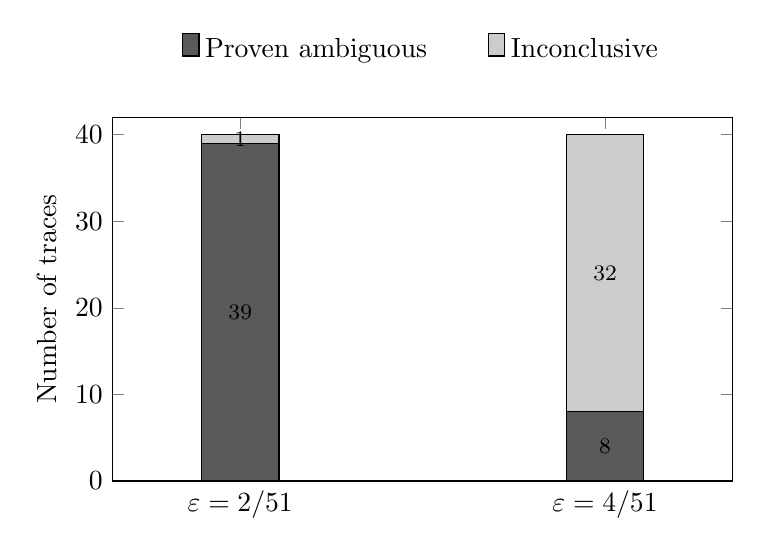
\begin{tikzpicture}
\begin{axis}[
  ybar stacked,
  bar width=28pt,
  width=0.78\linewidth,
  height=6.2cm,
  ymin=0,ymax=42,
  ylabel={Number of traces},
  symbolic x coords={$\varepsilon=2/51$,$\varepsilon=4/51$},
  xtick=data,
  legend style={at={(0.5,1.12)},anchor=south,legend columns=2,draw=none,/tikz/every even column/.append style={column sep=7mm}},
  nodes near coords,
  every node near coord/.append style={font=\footnotesize,text=black},
  enlarge x limits=0.35
]
\addplot+[draw=black,fill=black!65] coordinates {($\varepsilon=2/51$,39) ($\varepsilon=4/51$,8)};
\addplot+[draw=black,fill=black!20] coordinates {($\varepsilon=2/51$,1) ($\varepsilon=4/51$,32)};
\legend{Proven ambiguous,Inconclusive}
\end{axis}
\end{tikzpicture}
\caption{Opposite-answer completion witnesses by TV radius at the fixed immediate pre-stopping prefixes. Dark bars show traces proven ambiguous by explicit opposite-answer completion witnesses; light bars show the remaining inconclusive traces. Counts correspond to the fixed traces in Table~\ref{tab:witnesses}.}
\label{fig:witness_radius}
\end{figure}

The remaining 33 traces are inconclusive because failure to find an opposite-answer witness does not establish semantic agreement. Appendix~\ref{app:witness} records the witness construction and trace-level decision-point ledger.

\subsection{Result 3: conditional fixed-trace decision-point match}

For a fixed disclosure order, let $h_q$ denote the prefix containing the first $q$ disclosed fold vectors and define the first semantically resolving disclosure count, when it exists, by
\begin{equation}\label{eq:qstar}
q^\star=\min\left\{q:\mathcal D(X)\text{ is constant over all }X\in\mathcal X(h_q)\right\}.
\end{equation}
For every one of the 47 traces with a verified opposite-answer pair at $Q-1$, semantic resolution is impossible at $Q-1$ and at every earlier prefix of the same disclosure order, because the same two completions remain compatible when fewer observations are disclosed. The verified certificate at $Q$ provides the matching upper bound. The archived verification record therefore establishes a conditional fixed-trace lower/upper match on all 47 witnessed traces: $q^\star=Q$, subject to the original finite-well-defined-target scope and the numerical mean-enclosure qualification of the $Q$ certificate. Appendix~\ref{app:witness} reports these matches by disclosure policy and TV radius.

This is a fixed-order information statement, not an optimization over alternative disclosure orders. On these 47 traces, it distinguishes lack of earlier stopping caused by insufficient information from lack of earlier stopping caused by the tested certificate family.

\subsection{Verification of the real-data witnesses}

OpenAI ChatGPT and Codex assisted author-supervised code development and review. They were not used as independent decision-makers for reported labels or claims; numerical and logical results were retained only after the explicit verification checks described here and in Appendix~\ref{app:witness}.

The second completion rule was checked by a separately implemented verifier. Across all retained candidate completions, it checked agreement on disclosed values, declared score domains, mean-enclosure bounds, valid rank values, and file digests. The verification record contains 14,560 candidate support comparisons and 364 comparisons against the archived completion, together with per-task recipe and exact-tie diagnostics. Exact integer support signs determine acceptance; numerical linear-programming solves are diagnostic rather than the source of the logical label.

Because the verifier reuses the same parser and aggregation routines as the analysis, it serves as an implementation cross-check. Appendix~\ref{app:witness} records the verification scope and checks.

\subsection{Diagnostic interpretation}

Theorems~\ref{thm:nonuniform} and~\ref{thm:uniform} and the real-data witnesses diagnose complementary failure modes within the same decision problem.

\textbf{Certificate-expressiveness limit:} every legal completion has the same decision, but the restricted completion-independent certificate cannot express that fact. Additional evaluation is not logically required; a richer certificate may suffice.

\textbf{Information limit:} the same disclosed real benchmark transcript admits two legal completions with opposite decisions. No sound certificate can identify a unique answer from that transcript alone; additional information or stronger assumptions are required.

This distinction is the practical implication of the paper. Table~\ref{tab:diagnostic} summarizes the two unresolved failure modes that imply different remedies; Figure~\ref{fig:diagnostic_logic} additionally shows the certified and inconclusive outcomes needed for a sound diagnostic workflow. The zero-savings result separates diagnostic expressiveness from stopping-time performance.

\begin{table}[H]
\centering
\caption{Diagnostic interpretation of the two unresolved failure modes.}
\label{tab:diagnostic}
\begin{tabular}{>{\raggedright\arraybackslash}p{0.22\linewidth}>{\raggedright\arraybackslash}p{0.34\linewidth}>{\raggedright\arraybackslash}p{0.34\linewidth}}
\toprule
Aspect & Certificate-limited state & Information-limited state\\
\midrule
Compatible completions & All give the same decision & At least two give opposite decisions\\
What is insufficient & Restricted certificate family & Available benchmark evidence\\
Appropriate response & Use richer reasoning or a richer certificate & Collect more evidence or strengthen assumptions\\
\bottomrule
\end{tabular}
\end{table}

\section{Discussion and implications}

The exact constructions and the real-data study answer different questions. The constructions establish that semantic determination does not imply certifiability by the restricted family studied here. The real-data witnesses establish that unresolved real benchmark prefixes can also be genuinely information-limited. The practical distinction is therefore not simply whether an analysis has stopped, but why it cannot yet justify a decision.

For benchmark practitioners, the framework acts as a decision-support layer around incomplete evaluation. First ask whether two completions consistent with every disclosed evaluation can reverse the decision. If they can, additional evidence or stronger assumptions are unavoidable. If no such witness is found, certainty still does not follow; semantic determination must be established before certificate failure can be diagnosed. This ordering separates certificate design from information acquisition and prevents a failed witness search from being mistaken for agreement.

The zero-savings result shows that greater certificate expressiveness and lower evaluation effort are distinct objectives. In this study, the tested stronger family improves diagnostic interpretation rather than stopping time. For the 47 witnessed traces, the fixed-trace result $q^\star=Q$ goes further: under the recorded disclosure order and stated numerical scope, no sound procedure using the same evidence and assumptions can resolve the decision before $Q$.

The radius split is descriptive. Opposite-answer witnesses are found on 39 of 40 traces at $\varepsilon=2/51$ but only 8 of 40 at $\varepsilon=4/51$. Because the traces overlap within one archive, the contrast is not a statistical effect estimate. It shows that the geometry of the task-weight neighborhood materially changes which partial transcripts can be certified as ambiguous.

\section{Limitations}

The empirical analysis uses one benchmark archive, and the 80 traces overlap; their counts are descriptive rather than population estimates.

The completion domains are logical numerical domains. Compatible completions are not guaranteed to be realizable by retraining the named machine-learning methods.

The tested certificate family and opposite-answer search are not exhaustive. The 33 traces without a verified ambiguity witness therefore remain inconclusive. The fixed-trace $q^\star=Q$ result applies only to the 47 witnessed traces, the recorded disclosure order, finite well-defined canonical targets, and the mean-enclosure-qualified $Q$ certificate.

\section{Conclusion}

Incomplete machine-learning leaderboards can fail to support a decision for logically different reasons, and the remedy should depend on which failure mode is established. The decision-diagnostic framework labels a state information-limited when opposite-answer compatible completions are verified, certificate-limited only when semantic determination is established and nonexistence of a valid certificate in the declared family is proved, and inconclusive otherwise. The exact constructions establish the certificate-limited possibility, including the 68-task uniform construction. In the TabArena study, 47 of 80 immediate pre-stopping prefixes are information-limited. On all 47 witnessed traces, the $Q-1$ ambiguity witness and the verified $Q$ certificate yield the conditional fixed-trace match $q^\star=Q$ within the stated numerical scope; the other 33 traces remain inconclusive. The tested certificate strengthening provides no earlier stopping across 480 sampled checkpoints.

The practical implication is to diagnose the source of uncertainty before spending more benchmark-evaluation effort. If compatible completions disagree, more evidence or stronger assumptions are required. If the decision is proved fixed and the declared certificate family is proved insufficient, the appropriate target is richer reasoning. If neither condition is established, the system should report uncertainty. An unresolved leaderboard should therefore not be treated as synonymous with an under-evaluated leaderboard.


\appendix
\counterwithin{equation}{section}
\counterwithin{figure}{section}
\counterwithin{table}{section}
\renewcommand{\theequation}{\Alph{section}.\arabic{equation}}
\renewcommand{\thefigure}{\Alph{section}.\arabic{figure}}
\renewcommand{\thetable}{\Alph{section}.\arabic{table}}

\section{Detailed proof of the four-task obstruction}\label{app:fourtask}
The nonuniform construction in Theorem~\ref{thm:nonuniform} uses four methods labeled A--D and four tasks, nominal task weights $p=(21,21,21,5)/68$, and $\varepsilon=13/400$. One task is partially observed and three are fully observed. All raw losses lie in $[0,1]$, aggregation is the exact arithmetic mean, and ties use exact normalized midranks.

For the uncertain task, write the normalized ranks of B, C, and D as $(r_B,r_C,r_D)$ while A has rank 1. The six feasible triples are
\begin{equation}\label{eq:app_types}
(0,\tfrac13,\tfrac23),\;(\tfrac13,0,\tfrac23),\;(\tfrac16,\tfrac16,\tfrac23),\;(0,\tfrac12,\tfrac12),\;(\tfrac12,0,\tfrac12),\;(\tfrac13,\tfrac13,\tfrac13).
\end{equation}
All are realizable by the declared closed mean intervals. In every row, $r_B+r_C+r_D=1$ and $r_D\ge 1/3$.

To exclude A in every completion at the nominal weights, define $g=(1-r_B,1-r_C,1-r_D)$ and $t=(5/6,2/3,1/2)$. The three A-minus-rival nominal gaps are
\begin{equation}\label{eq:app_vj}
v_j=\frac{21}{68}(g_j-t_j)-\frac{5}{102}.
\end{equation}
Both $g$ and $t$ sum to 2, but $t$ is not one of the feasible $g$ vectors and all feasible coordinates lie on the $1/6$ lattice. Hence some coordinate satisfies $g_j-t_j\ge 1/6$, which gives
\begin{equation}\label{eq:app_A_margin}
\max_j v_j\ge \frac{21}{68\cdot6}-\frac{5}{102}=\frac1{408}>0.
\end{equation}
Thus A is excluded in every legal completion.

Each of B, C, and D is excluded by a feasible TV transfer of mass $\varepsilon=13/400$. The largest possible A-minus-rival gaps after the stated transfers are, respectively,
\begin{equation}\label{eq:app_nonA_gaps}
-\frac{211}{4080},\qquad -\frac{1}{4080},\qquad -\frac{211}{4080},
\end{equation}
so every non-A candidate is strictly defeated by A somewhere in the admissible TV neighborhood. Therefore every compatible completion has no common weak winner.

To show that no completion-independent joint mixture can uniformly exclude A, consider two legal uncertain-task mean rows $z_1=(3/4,0,1/8,1/4)$ and $z_2=(3/4,1/4,1/4,1/4)$. On the arithmetic average of their rank tables, the maximum A-minus-rival supports over the TV neighborhood are
\begin{equation}\label{eq:app_convex_supports}
-\frac{11}{40800},\qquad -\frac{29}{5100},\qquad -\frac{11}{40800}
\end{equation}
for B, C, and D. For any fixed probability mixture $\mu$ over admissible $(w,j)$ actions, linearity of the payoff in the rank table implies
\begin{equation}\label{eq:app_mixture}
\frac{F_\mu(z_1)+F_\mu(z_2)}2<0.
\end{equation}
At least one of the two legal completions must consequently have $F_\mu(z)<0$. Hence no fixed completion-independent mixture succeeds on every compatible completion, even though the semantic no-common-weak-winner decision has already been proved for every completion. The convexified average is used only in the impossibility argument; it is not assumed to be a realizable raw completion.

The public proof and replay materials record the corresponding exact-evidence and machine-audit artifacts; the proof uses only the declared synthetic construction and exact/rational checks.

\section{Uniform 68-task construction and exact verification}\label{app:uniform}
The stronger construction in Theorem~\ref{thm:uniform} uses four methods labeled A--D, 68 equally weighted tasks, and $\varepsilon=13/400$. The tasks form four blocks of sizes 21, 21, 21, and 5. The first block contains 21 independently incomplete tasks; the remaining 47 tasks are fully known. Each uncertain task can take one of six feasible rank-row types. Figure~\ref{fig:app_structure} shows the block structure and symmetry reduction.

\begin{figure}[H]
\centering
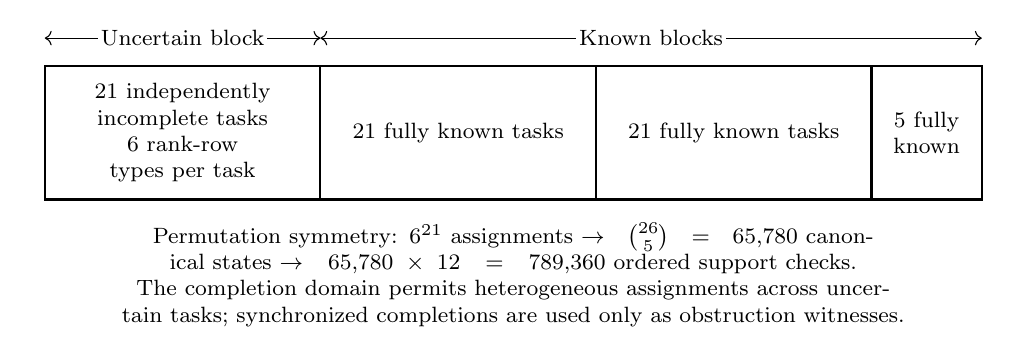
\begin{tikzpicture}[font=\footnotesize]
\def\h{1.70}
\draw[thick] (0,0) rectangle (3.5,\h);
\draw[thick] (3.5,0) rectangle (7.0,\h);
\draw[thick] (7.0,0) rectangle (10.5,\h);
\draw[thick] (10.5,0) rectangle (11.9,\h);
\node[align=center,text width=3.2cm] at (1.75,0.85) {21 independently incomplete tasks\\6 rank-row types per task};
\node[align=center,text width=3.1cm] at (5.25,0.85) {21 fully known tasks};
\node[align=center,text width=3.1cm] at (8.75,0.85) {21 fully known tasks};
\node[align=center,text width=1.2cm] at (11.2,0.85) {5 fully\\known};
\draw[<->] (0,2.05)--(3.5,2.05) node[midway,fill=white,inner sep=1pt]{Uncertain block};
\draw[<->] (3.5,2.05)--(11.9,2.05) node[midway,fill=white,inner sep=1pt]{Known blocks};
\node[align=center,text width=12.1cm] at (5.95,-0.95) {Permutation symmetry: $6^{21}$ assignments $\rightarrow \binom{26}{5}=65{,}780$ canonical states $\rightarrow 65{,}780\times12=789{,}360$ ordered support checks.\\The completion domain permits heterogeneous assignments across uncertain tasks; synchronized completions are used only as obstruction witnesses.};
\end{tikzpicture}
\caption{Structure of the 68-task uniform construction. The first 21 tasks are independently incomplete and each admits one of six feasible uncertain rank-row types. Permutation symmetry reduces the full $6^{21}$ assignment space to $\binom{26}{5}=65{,}780$ canonical states, and each state contributes 12 ordered candidate--rival support checks, yielding $789{,}360$ checks in total.}
\label{fig:app_structure}
\end{figure}

The completion domain permits heterogeneous assignments across the 21 uncertain tasks. Synchronized uncertain tasks are used only to exhibit obstruction witnesses and are not imposed on the completion domain. Because the nominal center is uniform, permuting the 21 uncertain tasks preserves every ordered-pair support. The $6^{21}$ possible rank tables therefore reduce to the weak compositions of 21 items into six types, giving $\binom{26}{5}=65{,}780$ canonical states.

The independent exact checker evaluates 12 ordered candidate--rival comparisons for each canonical state,
\begin{equation}\label{eq:app_checks}
65{,}780\times12=789{,}360\text{ ordered support comparisons.}
\end{equation}
All 63 nonempty subsets of the six uncertain row types were also checked. Exact integer transport and a separate rational-arithmetic implementation agree on the support signs. A fresh replay on Python 3.13.5 reproduced the same verification outcome obtained previously on Python 3.12.14. The archived uniform-construction verification artifact used in that replay has SHA-256 \url{ca61a164846342f5489cbbf3c9f068b3d1d76e8314ff549f46288b57de6fcd50}.

\section{Real-data witness ledger and fixed-trace verification}\label{app:witness}
For each empirical trace, $Q$ is the recorded stopping disclosure count and the information-limitation analysis examines $Q-1$. The archived completion supplies one decision label. Constructed completions use only disclosed observations and the declared score domains; the actual unseen fold values and unseen decision label are not inputs to the construction.

The initial constant-fill recipe supplied witnesses on 36 of 80 traces. A second prespecified equalization-based recipe retained all 36 and raised the total to 47. The second rule evaluated 14 candidate completions per trace across all 80 traces, yielding 1,120 candidate-completion trials. Table~\ref{tab:app_qmatch} reports the fixed-trace $q^\star=Q$ matches by disclosure policy and TV radius.

\begin{table}[H]
\centering
\caption{Conditional fixed-trace decision-point matches by disclosure policy and TV radius. A match combines a verified ambiguity witness at $Q-1$ with the verified stopping-prefix certificate at $Q$.}
\label{tab:app_qmatch}
\footnotesize
\begin{tabular}{lrrr}
\toprule
Disclosure policy & TV radius & Traces & $q^\star=Q$ matches\\
\midrule
Random fold & $2/51$ & 10 & 10\\
Random fold & $4/51$ & 10 & 1\\
Random task blocks & $2/51$ & 10 & 9\\
Random task blocks & $4/51$ & 10 & 3\\
Cheapest remaining & $2/51$ & 10 & 10\\
Cheapest remaining & $4/51$ & 10 & 2\\
Decision gap & $2/51$ & 10 & 10\\
Decision gap & $4/51$ & 10 & 2\\
\midrule
Total & --- & 80 & 47\\
\bottomrule
\end{tabular}
\end{table}

For the same fixed disclosure order, the verified opposite-answer pair at $Q-1$ gives $q^\star>Q-1$. The verified certificate at $Q$ gives $q^\star\le Q$, subject to the finite-well-defined-target scope and the numerical mean-enclosure qualification. Hence all 47 successful witness traces satisfy the conditional fixed-trace match $q^\star=Q$. This statement does not compare alternative query orders.

A separately implemented verifier checked agreement on disclosed values, declared score domains, mean-enclosure bounds, valid rank values, exact-tie handling, and file digests. The verification record contains 14,560 candidate support comparisons and 364 comparisons against the archived completion. Exact integer support signs determine witness acceptance; numerical linear-programming solves are diagnostic. Because the verifier reuses the same parser and aggregation routines as the analysis, it is an implementation cross-check rather than an independent replication.

The public repository at \url{https://github.com/shaikhamalkawi-ux/decision-diagnosis-incomplete-ml-leaderboards} contains the diagnostic procedure, detailed proof materials, result summaries, the fixed-trace verifier and summary, figure-reproduction code, and provenance notes. Third-party raw TabArena artifacts are not redistributed where redistribution rights are unclear; retrieval and provenance information are supplied instead.


\section*{Declaration of generative AI and AI-assisted technologies in the manuscript preparation process}
During the preparation of this work, the authors used OpenAI ChatGPT and Codex to assist with literature searching, manuscript organization and language editing, code development and review, and reproducibility checks. After using these tools, the authors reviewed and edited the content as needed and take full responsibility for the content of the publication.

\section*{Data and reproducibility materials availability}
Reproducibility materials are publicly available at the following repository:\\
\url{https://github.com/shaikhamalkawi-ux/decision-diagnosis-incomplete-ml-leaderboards}.\\
The repository includes detailed proof materials for the exact obstruction constructions, exact-case evidence, executable verification code and tests, the diagnostic procedure, witness summaries, and the fixed-trace $q^\star=Q$ verification summary. Third-party raw TabArena artifacts are not redistributed where redistribution rights are unclear; provenance and retrieval instructions are provided instead. Dataset and benchmark provenance are documented following the transparency and reproducibility principles emphasized in \cite{r25,r26}.

\begin{thebibliography}{99}
\bibitem{r1} A. Himmi, E. Irurozki, N. Noiry, S. Cl\'emen\c{c}on and P. Colombo, Towards More Robust NLP System Evaluation: Handling Missing Scores in Benchmarks, in Findings of the Association for Computational Linguistics: EMNLP 2024 (2024), pp. 11759--11785, \url{https://doi.org/10.18653/v1/2024.findings-emnlp.688}.
\bibitem{r2} L. Xia and V. Conitzer, Determining possible and necessary winners under common voting rules given partial orders, J. Artif. Intell. Res. 41 (2011) 25--67, \url{https://doi.org/10.1613/jair.3186}.
\bibitem{r3} T. Lu and C. Boutilier, Preference elicitation and robust winner determination for single- and multi-winner social choice, Artif. Intell. 279 (2020) 103203, \url{https://doi.org/10.1016/j.artint.2019.103203}.
\bibitem{r4} D. Baumeister, M. Neveling, M. Roos, J. Rothe, L. Schend, R. Weishaupt and L. Xia, The possible winner with uncertain weights problem, J. Comput. Syst. Sci. 138 (2023) 103464, \url{https://doi.org/10.1016/j.jcss.2023.103464}.
\bibitem{r5} P. Viappiani, Robust winner determination in positional scoring rules with uncertain weights, Theory Decis. 88 (2020) 323--367, \url{https://doi.org/10.1007/s11238-019-09734-3}.
\bibitem{r6} R. O'Shea, P. Deeney, E. Triantaphyllou, L. Diaz-Balteiro and S. A. Tarim, Weight stability intervals for multi-criteria decision analysis using the weighted sum model, Expert Syst. Appl. 296 (2026) 128460, \url{https://doi.org/10.1016/j.eswa.2025.128460}.
\bibitem{r7} D. C. Parkes, Price-Based Information Certificates for Minimal-Revelation Combinatorial Auctions, in Agent-Mediated Electronic Commerce IV: Designing Mechanisms and Systems, Lecture Notes in Artificial Intelligence 2531 (Springer, 2002), pp. 103--122, \url{https://doi.org/10.1007/3-540-36378-5_7}.
\bibitem{r8} S. Corrente, S. Greco and R. S\l{}owi\'nski, Handling imprecise evaluations in multiple criteria decision aiding and robust ordinal regression by n-point intervals, Fuzzy Optim. Decis. Mak. 16 (2017) 127--157, \url{https://doi.org/10.1007/s10700-016-9244-x}.
\bibitem{r9} P. Vayanos, A. Georghiou and H. Yu, Robust optimization with decision-dependent information discovery, Manag. Sci. 72(2) (2025) 1509--1528, \url{https://doi.org/10.1287/mnsc.2021.00160}.
\bibitem{r10} S. Mishra and A. Arunkumar, How Robust are Model Rankings: A Leaderboard Customization Approach for Equitable Evaluation, Proc. AAAI Conf. Artif. Intell. 35(15) (2021) 13561--13569, \url{https://doi.org/10.1609/aaai.v35i15.17599}.
\bibitem{r11} P. Gordienko, G. Schollmeyer, F. Kreuter and C. Jansen, How Hard is it to Rig a Benchmark? A Social Choice Analysis of Leaderboard Robustness, arXiv:2605.23628 (2026), \url{https://doi.org/10.48550/arXiv.2605.23628}.
\bibitem{r12} N. Erickson, L. Purucker, A. Tschalzev, D. Holzm\"uller, P. M. Desai, D. Salinas and F. Hutter, TabArena: A Living Benchmark for Machine Learning on Tabular Data, Adv. Neural Inf. Process. Syst. 38, Datasets and Benchmarks Track (2025), pp. 17285--17350, \url{https://doi.org/10.52202/085713-0519}.
\bibitem{r13} J. Dem\v{s}ar, Statistical comparisons of classifiers over multiple data sets, J. Mach. Learn. Res. 7 (2006) 1--30, \url{https://www.jmlr.org/papers/v7/demsar06a.html}.
\bibitem{r14} A. Benavoli, G. Corani, J. Dem\v{s}ar and M. Zaffalon, Time for a change: a tutorial for comparing multiple classifiers through Bayesian analysis, J. Mach. Learn. Res. 18(77) (2017) 1--36, \url{https://www.jmlr.org/papers/v18/16-305.html}.
\bibitem{r15} X. Bouthillier, P. Delaunay, M. Bronzi, A. Trofimov, B. Nichyporuk, J. Szeto, N. Mohammadi Sepahvand, E. Raff, K. Madan, V. Voleti, S. Ebrahimi Kahou, V. Michalski, D. Serdyuk, T. Arbel, C. Pal, G. Varoquaux and P. Vincent, Accounting for variance in machine learning benchmarks, Proc. Mach. Learn. Syst. 3 (2021) 747--769, \url{https://proceedings.mlsys.org/paper/2021/hash/0184b0cd3cfb185989f858a1d9f5c1eb-Abstract.html}.
\bibitem{r16} J. Vanschoren, J. N. van Rijn, B. Bischl and L. Torgo, OpenML: networked science in machine learning, SIGKDD Explor. 15(2) (2013) 49--60, \url{https://doi.org/10.1145/2641190.2641198}.
\bibitem{r17} B. Bischl, G. Casalicchio, M. Feurer, P. Gijsbers, F. Hutter, M. Lang, R. G. Mantovani, J. N. van Rijn and J. Vanschoren, OpenML Benchmarking Suites, in Proc. Neural Information Processing Systems Track on Datasets and Benchmarks, Vol. 1 (2021), \url{https://datasets-benchmarks-proceedings.neurips.cc/paper/2021/hash/c7e1249ffc03eb9ded908c236bd1996d-Abstract-round2.html}.
\bibitem{r18} P. Gijsbers, M. L. P. Bueno, S. Coors, E. LeDell, S. Poirier, J. Thomas, B. Bischl and J. Vanschoren, AMLB: an AutoML Benchmark, J. Mach. Learn. Res. 25(101) (2024) 1--65, \url{https://www.jmlr.org/papers/v25/22-0493.html}.
\bibitem{r19} R. Lahdelma, J. Hokkanen and P. Salminen, SMAA---Stochastic multiobjective acceptability analysis, Eur. J. Oper. Res. 106(1) (1998) 137--143, \url{https://doi.org/10.1016/S0377-2217(97)00163-X}.
\bibitem{r20} R. Lahdelma and P. Salminen, SMAA-2: Stochastic Multicriteria Acceptability Analysis for Group Decision Making, Oper. Res. 49(3) (2001) 444--454, \url{https://doi.org/10.1287/opre.49.3.444.11220}.
\bibitem{r21} T. Tervonen and R. Lahdelma, Implementing stochastic multicriteria acceptability analysis, Eur. J. Oper. Res. 178(2) (2007) 500--513, \url{https://doi.org/10.1016/j.ejor.2005.12.037}.
\bibitem{r22} S. Greco, V. Mousseau and R. S\l{}owi\'nski, Ordinal regression revisited: multiple criteria ranking using a set of additive value functions, Eur. J. Oper. Res. 191(2) (2008) 416--436, \url{https://doi.org/10.1016/j.ejor.2007.08.013}.
\bibitem{r23} S. Greco, M. Kadzi\'nski, V. Mousseau and R. S\l{}owi\'nski, ELECTRE$^{\mathrm{GKMS}}$: robust ordinal regression for outranking methods, Eur. J. Oper. Res. 214(1) (2011) 118--135, \url{https://doi.org/10.1016/j.ejor.2011.03.045}.
\bibitem{r24} S. Greco, R. S\l{}owi\'nski and J. Wallenius, Fifty years of multiple criteria decision analysis: from classical methods to robust ordinal regression, Eur. J. Oper. Res. 323(2) (2025) 351--377, \url{https://doi.org/10.1016/j.ejor.2024.07.038}.
\bibitem{r25} T. Gebru, J. Morgenstern, B. Vecchione, J. Wortman Vaughan, H. Wallach, H. Daum\'e III and K. Crawford, Datasheets for datasets, Commun. ACM 64(12) (2021) 86--92, \url{https://doi.org/10.1145/3458723}.
\bibitem{r26} J. Pineau, P. Vincent-Lamarre, K. Sinha, V. Larivi\`ere, A. Beygelzimer, F. d'Alch\'e-Buc, E. Fox and H. Larochelle, Improving Reproducibility in Machine Learning Research (A Report from the NeurIPS 2019 Reproducibility Program), J. Mach. Learn. Res. 22(164) (2021) 1--20, \url{https://www.jmlr.org/papers/v22/20-303.html}.
\end{thebibliography}


\end{document}